\documentclass{article}

\usepackage{fancyhdr}
\usepackage{extramarks}
\usepackage{amsmath}
\usepackage{amssymb}
\usepackage{amsthm}
\usepackage{amsfonts}
\usepackage{tikz}
\usepackage[plain]{algorithm}
\usepackage{algpseudocode}

\usetikzlibrary{automata,positioning}

%
% Basic Document Settings
%

\topmargin=-0.45in
\evensidemargin=0in
\oddsidemargin=0in
\textwidth=6.5in
\textheight=9.0in
\headsep=0.25in

\linespread{1.1}

\pagestyle{fancy}
\lhead{\hmwkAuthorName}
\chead{\hmwkClass\ (\hmwkClassInstructor): \hmwkTitle}
\rhead{\firstxmark}
\lfoot{\lastxmark}
\cfoot{\thepage}

\renewcommand\headrulewidth{0.4pt}
\renewcommand\footrulewidth{0.4pt}

\setlength\parindent{0pt}

%
% Create Problem Sections
%

\newcommand{\enterProblemHeader}[1]{
    \nobreak\extramarks{}{Question \arabic{#1} continued on next page\ldots}\nobreak{}
    \nobreak\extramarks{Question \arabic{#1} (continued)}{Question \arabic{#1} continued on next page\ldots}\nobreak{}
}

\newcommand{\exitProblemHeader}[1]{
    \nobreak\extramarks{Question \arabic{#1} (continued)}{Question \arabic{#1} continued on next page\ldots}\nobreak{}
    \stepcounter{#1}
    \nobreak\extramarks{Question \arabic{#1}}{}\nobreak{}
}

\setcounter{secnumdepth}{0}
\newcounter{partCounter}
\newcounter{homeworkProblemCounter}
\setcounter{homeworkProblemCounter}{1}
\nobreak\extramarks{Question \arabic{homeworkProblemCounter}}{}\nobreak{}

%
% Homework Problem Environment
%
% This environment takes an optional argument. When given, it will adjust the
% problem counter. This is useful for when the problems given for your
% assignment aren't sequential. See the last 3 problems of this template for an
% example.
%
\newenvironment{homeworkProblem}[1][-1]{
    \ifnum#1>0
        \setcounter{homeworkProblemCounter}{#1}
    \fi
    \section{Question \arabic{homeworkProblemCounter}}
    \setcounter{partCounter}{1}
    \enterProblemHeader{homeworkProblemCounter}
}{
    \exitProblemHeader{homeworkProblemCounter}
}

%
% Homework Details
%   - Title
%   - Due date
%   - Class
%   - Section/Time
%   - Instructor
%   - Author
%

\newcommand{\hmwkTitle}{Assignment\ \#1}
\newcommand{\hmwkDueDate}{February 27, 2018}
\newcommand{\hmwkClass}{AIC}
% \newcommand{\hmwkClassTime}{}
\newcommand{\hmwkClassInstructor}{Dr. D. Seshachalam}
\newcommand{\hmwkAuthorName}{\textbf{A13}}

%
% Title Page
%

% \title{
%     \vspace{2in}
%     \textmd{\textbf{\hmwkClass:\ \hmwkTitle}}\\
%     \normalsize\vspace{0.1in}\small{Due\ on\ \hmwkDueDate\ at 3:10pm}\\
%     \vspace{0.1in}\large{\textit{\hmwkClassInstructor\ \hmwkClassTime}}
%     \vspace{3in}
% }

% \author{\hmwkAuthorName}
% \date{}

\renewcommand{\part}[1]{\textbf{\large Part \Alph{partCounter}}\stepcounter{partCounter}\\}

%
% Various Helper Commands
%

% Useful for algorithms
\newcommand{\alg}[1]{\textsc{\bfseries \footnotesize #1}}

% For derivatives
\newcommand{\deriv}[1]{\frac{\mathrm{d}}{\mathrm{d}x} (#1)}

% For partial derivatives
\newcommand{\pderiv}[2]{\frac{\partial}{\partial #1} (#2)}

% Integral dx
\newcommand{\dx}{\mathrm{d}x}

% Alias for the Solution section header
\newcommand{\solution}{\textbf{\large Solution}}

% Probability commands: Expectation, Variance, Covariance, Bias
\newcommand{\E}{\mathrm{E}}
\newcommand{\Var}{\mathrm{Var}}
\newcommand{\Cov}{\mathrm{Cov}}
\newcommand{\Bias}{\mathrm{Bias}}

\begin{document}

\title{\fontsize{14pt}{16.8pt}\selectfont\bf{ANALOG INTEGRATED CIRCUITS [15ES4GCAIC]}}
\date{}

\maketitle
\thispagestyle{empty}

\begin{center}
\vspace*{-15mm}

{\fontsize{14pt}{16.8pt}\selectfont\textbf{SELF STUDY}} \\
\vspace*{4mm}

{\fontsize{14pt}{16.8pt}\selectfont\textit{in}} \\
\vspace*{3mm}

{\fontsize{14pt}{16.8pt}\selectfont\textbf{ELECTRONICS AND COMMUNICATION ENGINEERING}} \\

\vspace*{4mm}
{\fontsize{14pt}{16.8pt}\selectfont\textit{by}} \\
\vspace*{5mm}

\author{\fontsize{14pt}{16.8pt}\selectfont\textbf{A. Vipula}}  \hspace*{12mm} {\fontsize{14pt}{16.8pt}\selectfont\textbf{Akshit Bhalla}} \hspace*{12mm} {\fontsize{14pt}{16.8pt}\selectfont\textbf{Amrutha M.}}\\
\vspace*{2mm}
{\fontsize{12pt}{14.4pt}\selectfont\textit{[1BM16EC007]} \hspace*{12mm} \selectfont\textit{[1BM16EC015]} \hspace*{12mm} \selectfont\textit{[1BM16EC018]} } \\



\vspace*{3mm}

\vspace*{4mm}\fontsize{14pt}{16.8pt}\selectfont\textit{Under the supervision of} \\
\vspace*{2mm}\fontsize{14pt}{16.8pt}\selectfont\textbf{Dr. D. Seshachalam} \\
\vspace*{8mm}

\begin{figure}[!ht]
\centering
  
\includegraphics[height=36.068mm,width=33.274mm]{assets/BMSCE_Logo.png}
\end{figure}

\vspace*{3mm}

{\fontsize{14pt}{16.8pt}\selectfont\textbf{February 28th, 2018}} \\

\vspace*{5mm}

\fontsize{14pt}{16.8pt}\selectfont\textbf{Department of Electronics and Communication Engineering \\
\vspace*{4mm}
\vspace*{2mm} B.M.S COLLEGE OF ENGINEERING, Basavanagudi} \\
\vspace*{2mm}
\fontsize{14pt}{16.8pt}\selectfont\textbf{Bangalore-560019, India} 
\vspace*{10mm}\\

\end{center}
 % cover page
\thispagestyle{empty}
\newpage

% \maketitle

\graphicspath{{assets/}} % path to images folder

\pagebreak

\begin{homeworkProblem}
    Plot the frequency response curve for any practical circuit using 741 		op-amp and verify the following equation: 
    
    \vspace{5mm}
	\hspace{1cm} \((Bandwidth\ast Gain)_{open loop}\) = \((Bandwidth\ast Gain)_{closed loop}\)
    
    \vspace{5mm}
    \solution \\

	For Open Loop configuration, the \(Bandwidth\ast Gain = 5 \times 2 \times 10^5 = 1 MHz\) \\
    
    Gain is represented in decibels. 
   	\(Gain_{dB} = 20\log_{10} {Gain}\) \\
  We have used Bode plot to represent the plot of \(\lvert Gain \rvert\; vs.\; Frequency\)\\
  The circuit shown is an inverting amplifier.
    
    From the graph, in Closed Loop configuration:
    \begin{itemize}
  \item \(Bandwidth = 96.619 kHz\)
  \item \(Gain = 10^{22.973/20} = 14.081\)
\end{itemize} 

	\(\therefore (Bandwidth\ast Gain)_{closed loop} = 1.36 MHz \approx (Bandwidth\ast Gain)_{open loop}\)

    \begin{figure}[H] 
      \centering
      \resizebox{12cm}{6cm}{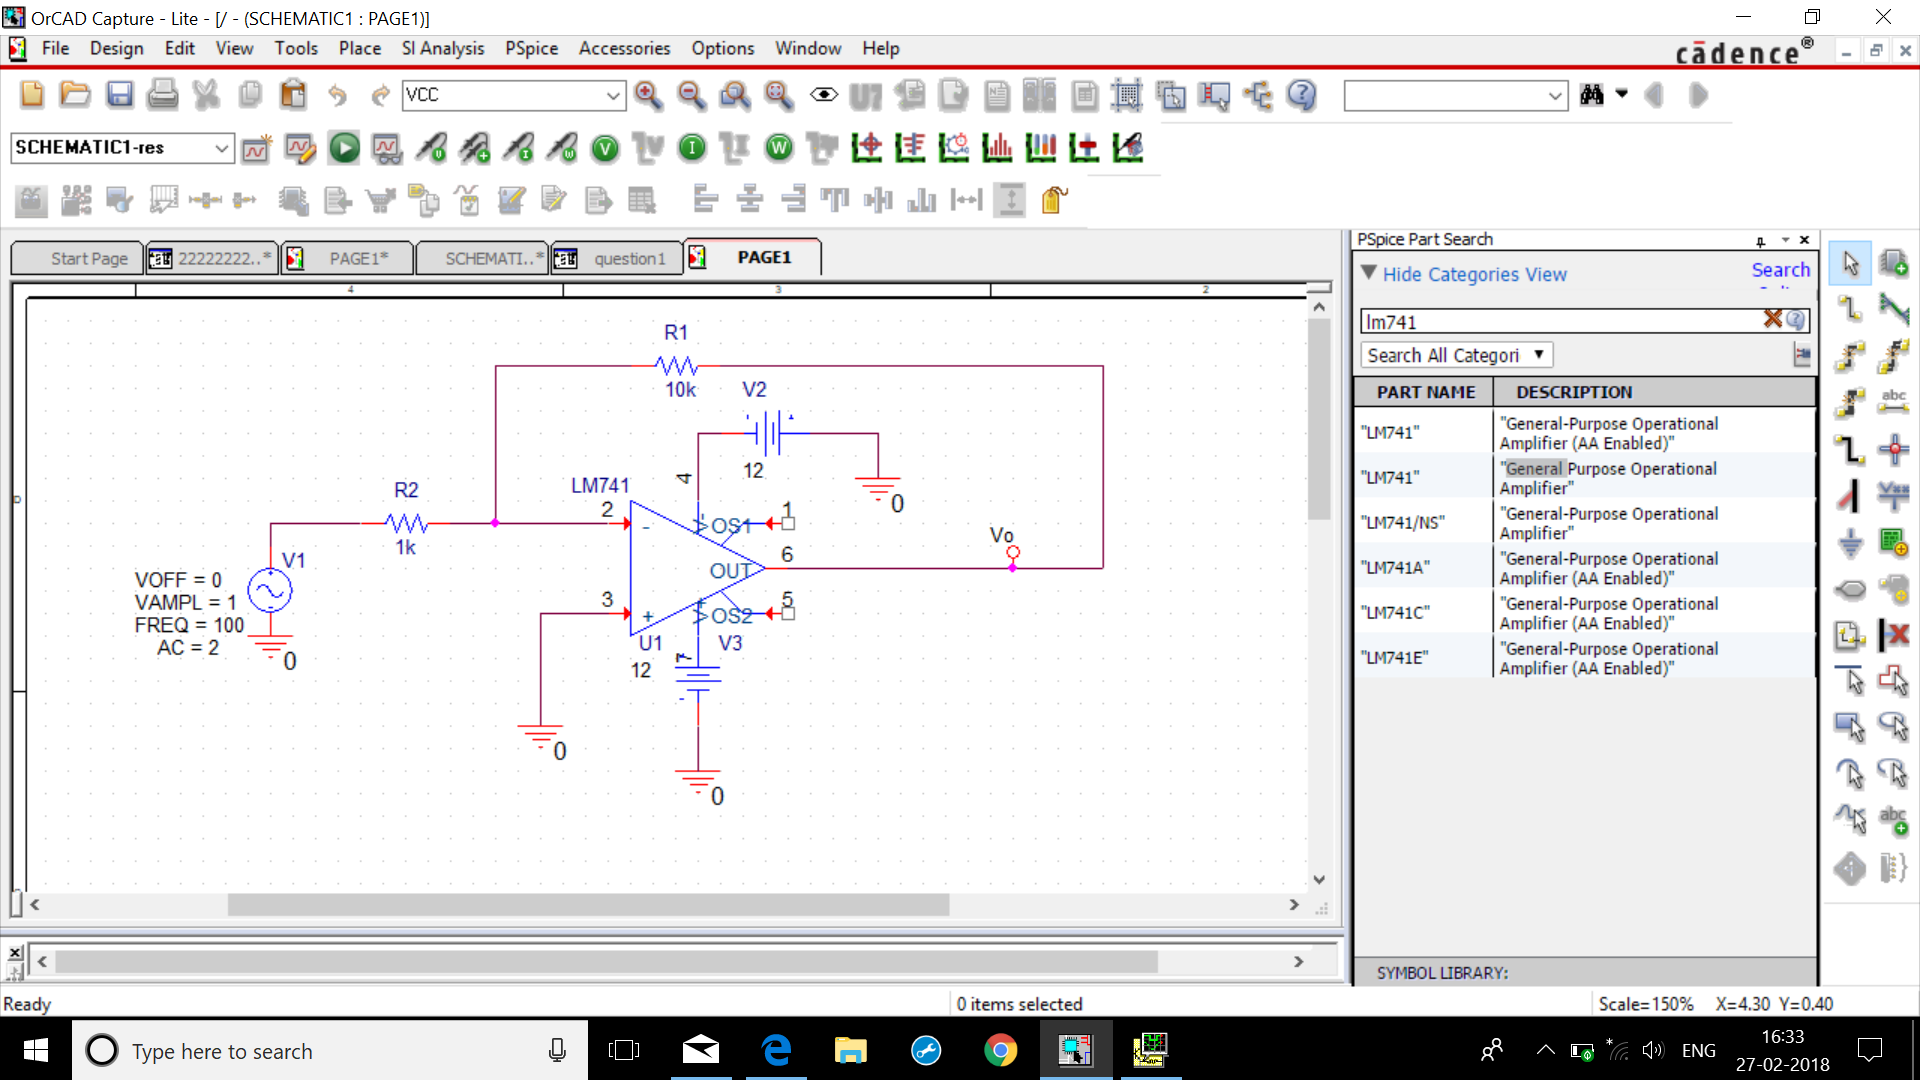
\includegraphics{Q1/circuit}}  7
      \centering
      \caption{Circuit Diagram}
      \label{fig:circuit}
	\end{figure}
    
    \begin{figure}[H] 
      \centering
       \resizebox{12cm}{6cm}{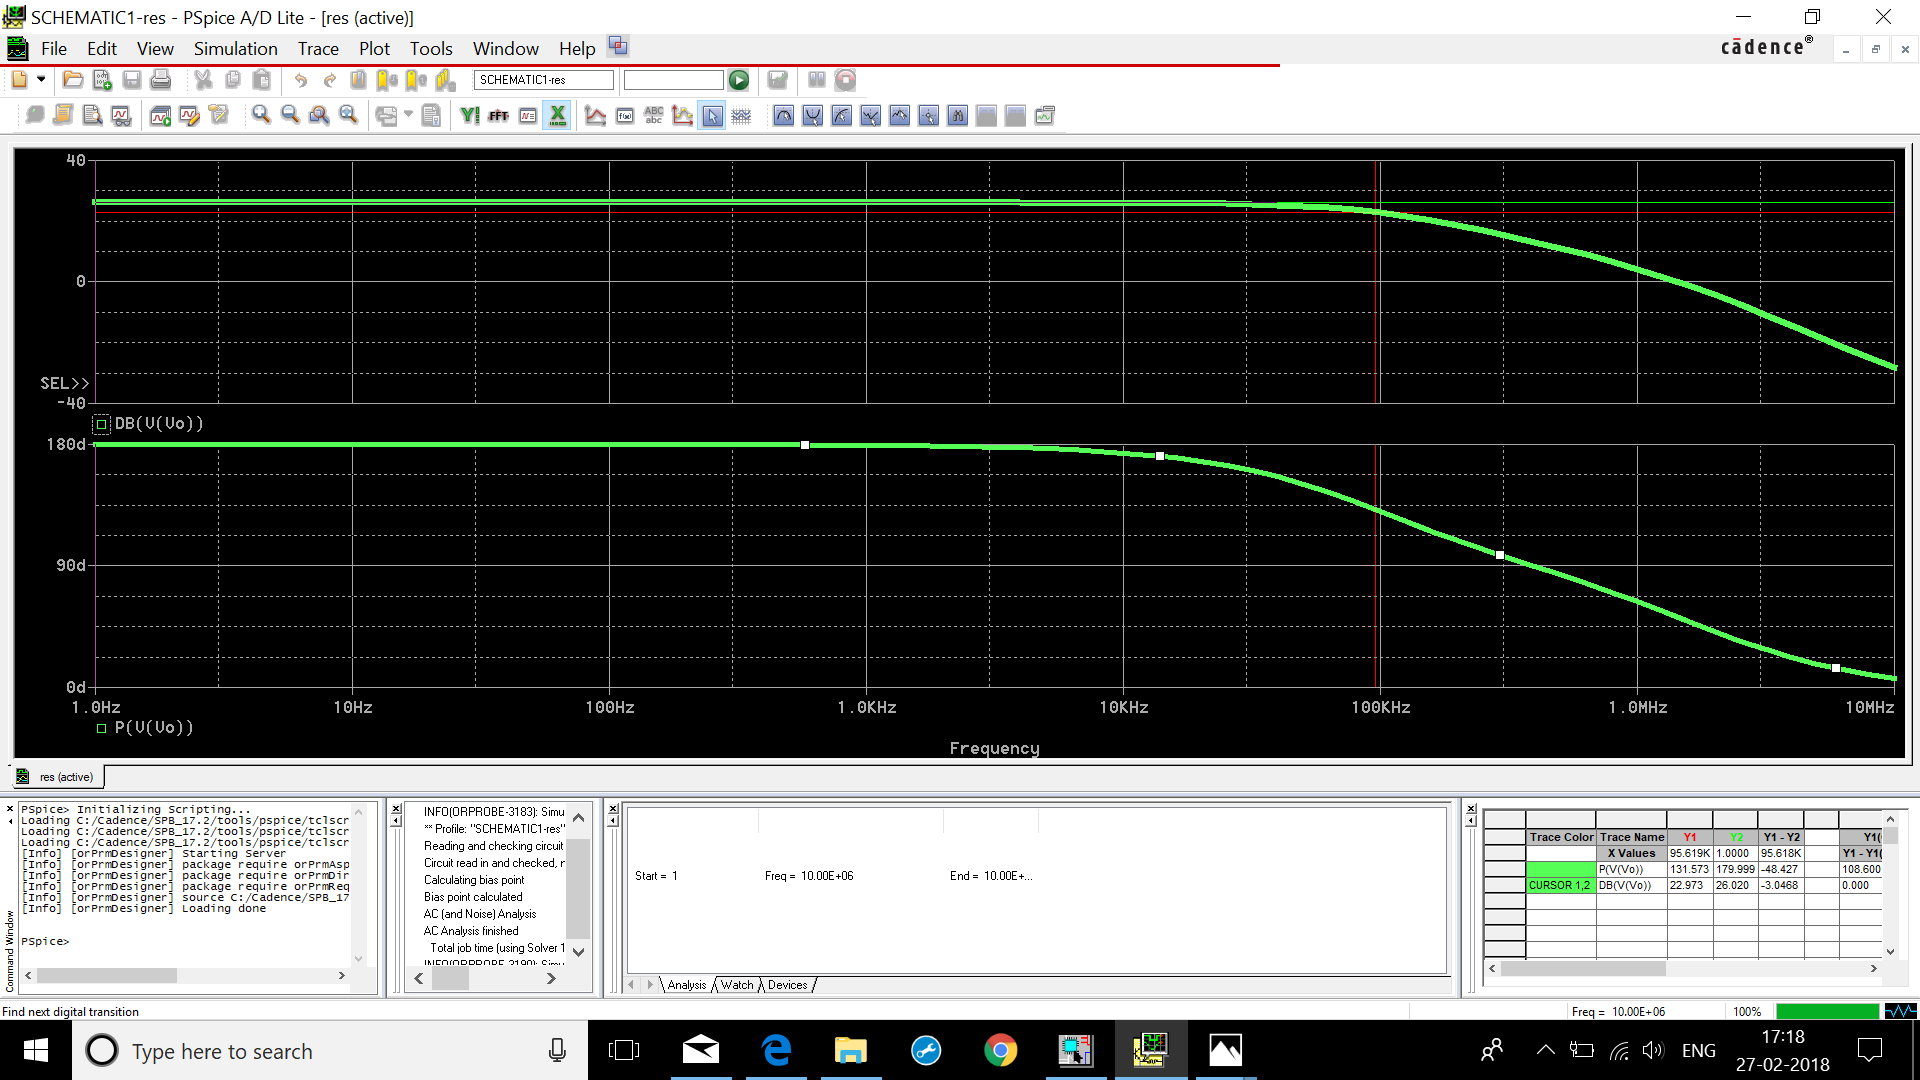
\includegraphics{Q1/graph}}  
      \centering
      \caption{Graph}
      \label{fig:graph}
	\end{figure}
    
\end{homeworkProblem}

\pagebreak

\begin{homeworkProblem}
    
    Calculate various DC and AC electrical parameters for a given OPAMP and verify the same with various datasheet.
    
    \vspace{5mm}
    \solution \\
    
    The Operational Amplifier used is LM358NS. Bias Point Analysis was performed in order to obtain the DC parameters of the circuit.Current and Voltage readings in every branch have been found.
    
    \begin{itemize}
  \item \(Input\:Bias\: Current\; I_B = \frac{-48.23 nA - 41.70 nA}{2} = - 44.965 nA\)
  \item \(Input\: Offset\: Current\; I_{OS} = -41.70 nA - (-48.23 nA) = 6.53 nA\)
  \item \(Input\: Offset\: Voltage\; V_{OS} = 3 mV,\; V_{Output} = 962.2 \mu V \approx 0 V\)
\end{itemize}
    
    The values obtained are verified as per the  datasheet given below.
    
    \begin{figure}[H] 
      \centering
      \resizebox{12cm}{6cm}{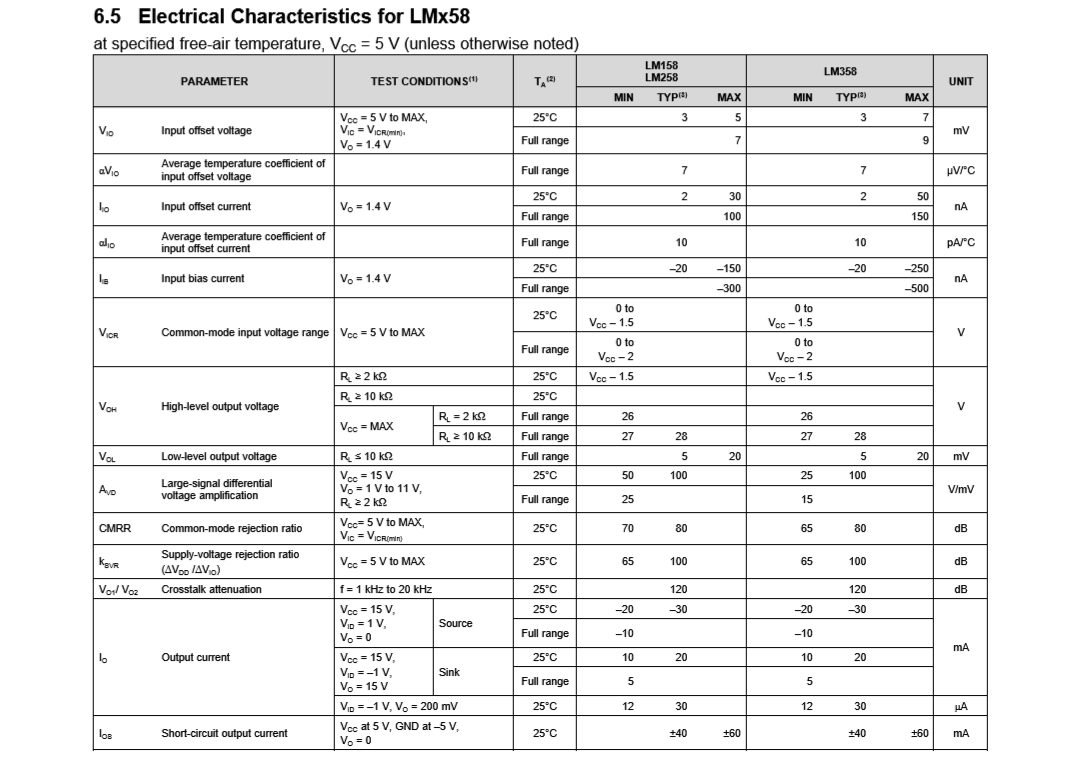
\includegraphics{LM358}}  
      \centering
      \caption{Datasheet of LM358 Operational Amplifier}
      \label{fig:LM358}
	\end{figure}
    
    \begin{figure}[H] 
      \centering
      \resizebox{12cm}{6cm}{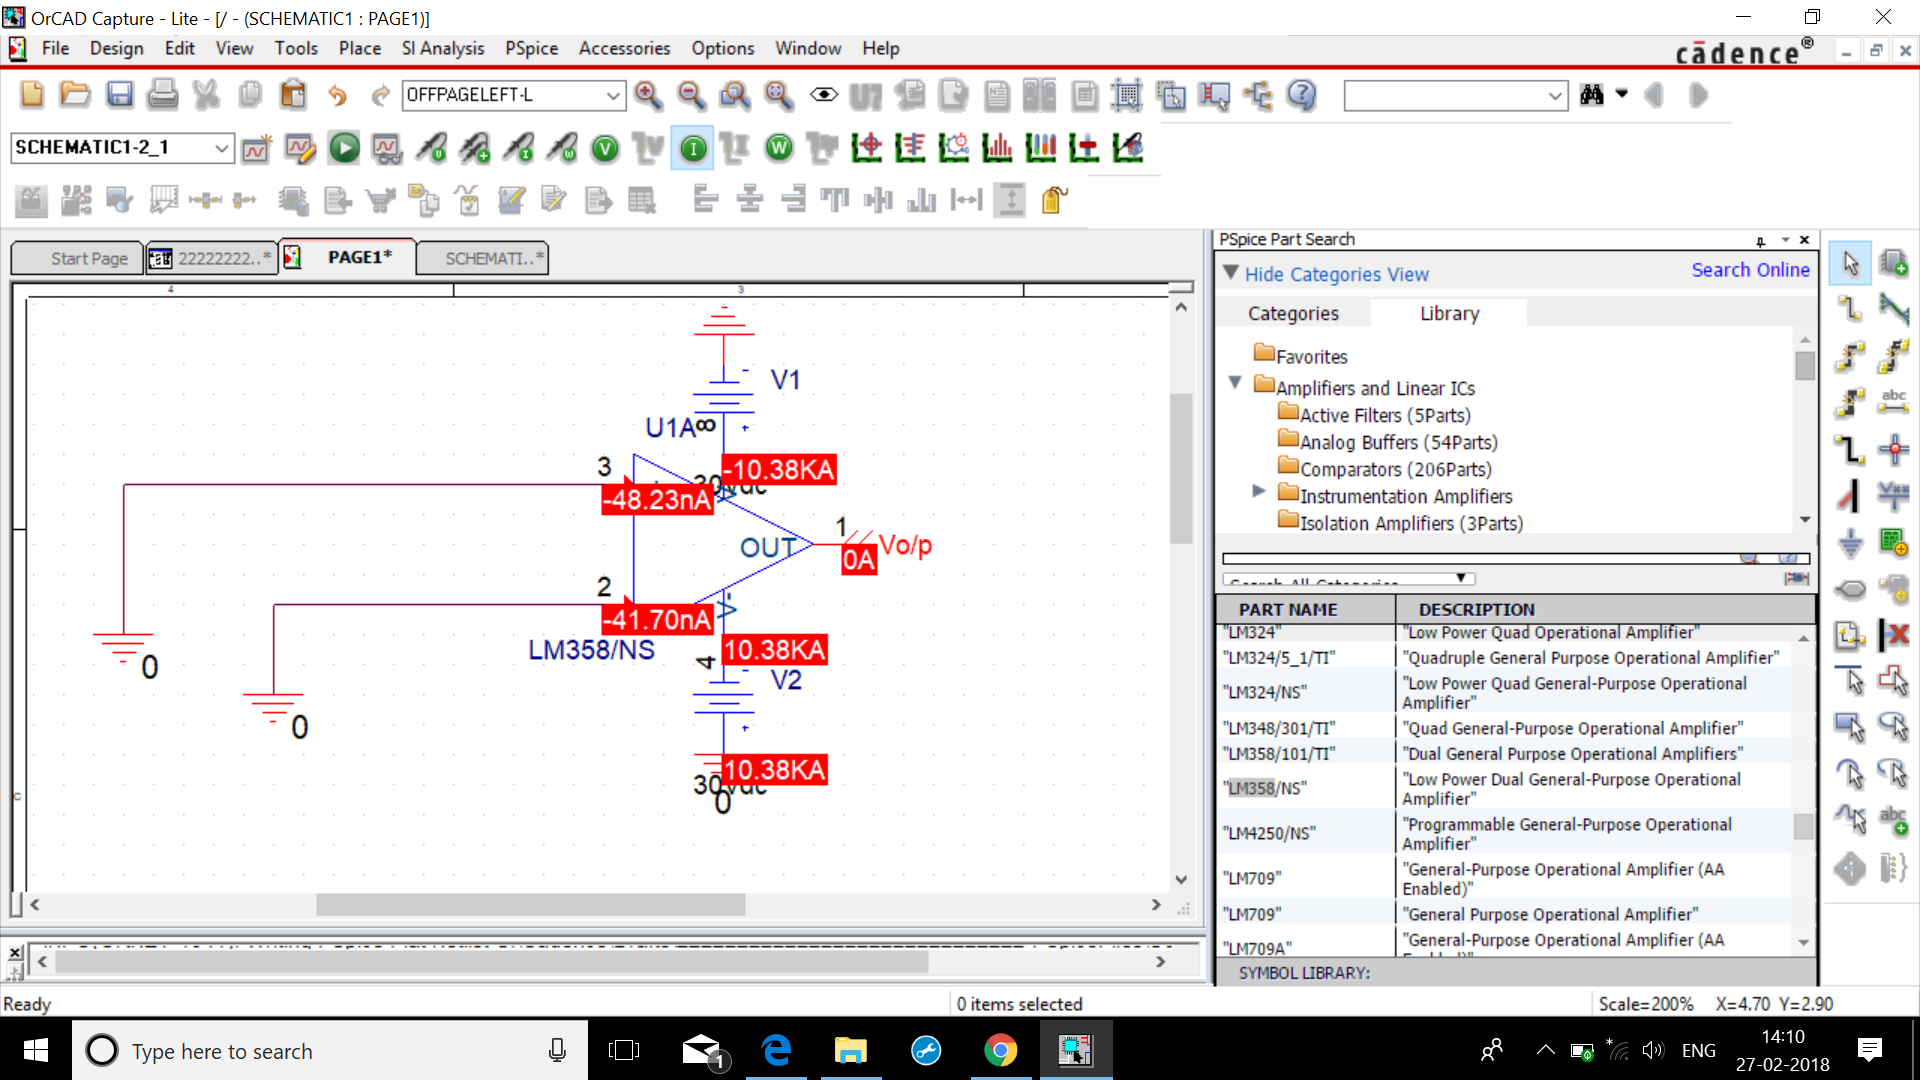
\includegraphics{Q2/offset_current}}  
      \centering
      \caption{Circuit Diagram with Current Markers}
      \label{fig:offset_current}
	\end{figure}
    
    \begin{figure}[H] 
      \centering
      \resizebox{12cm}{6cm}{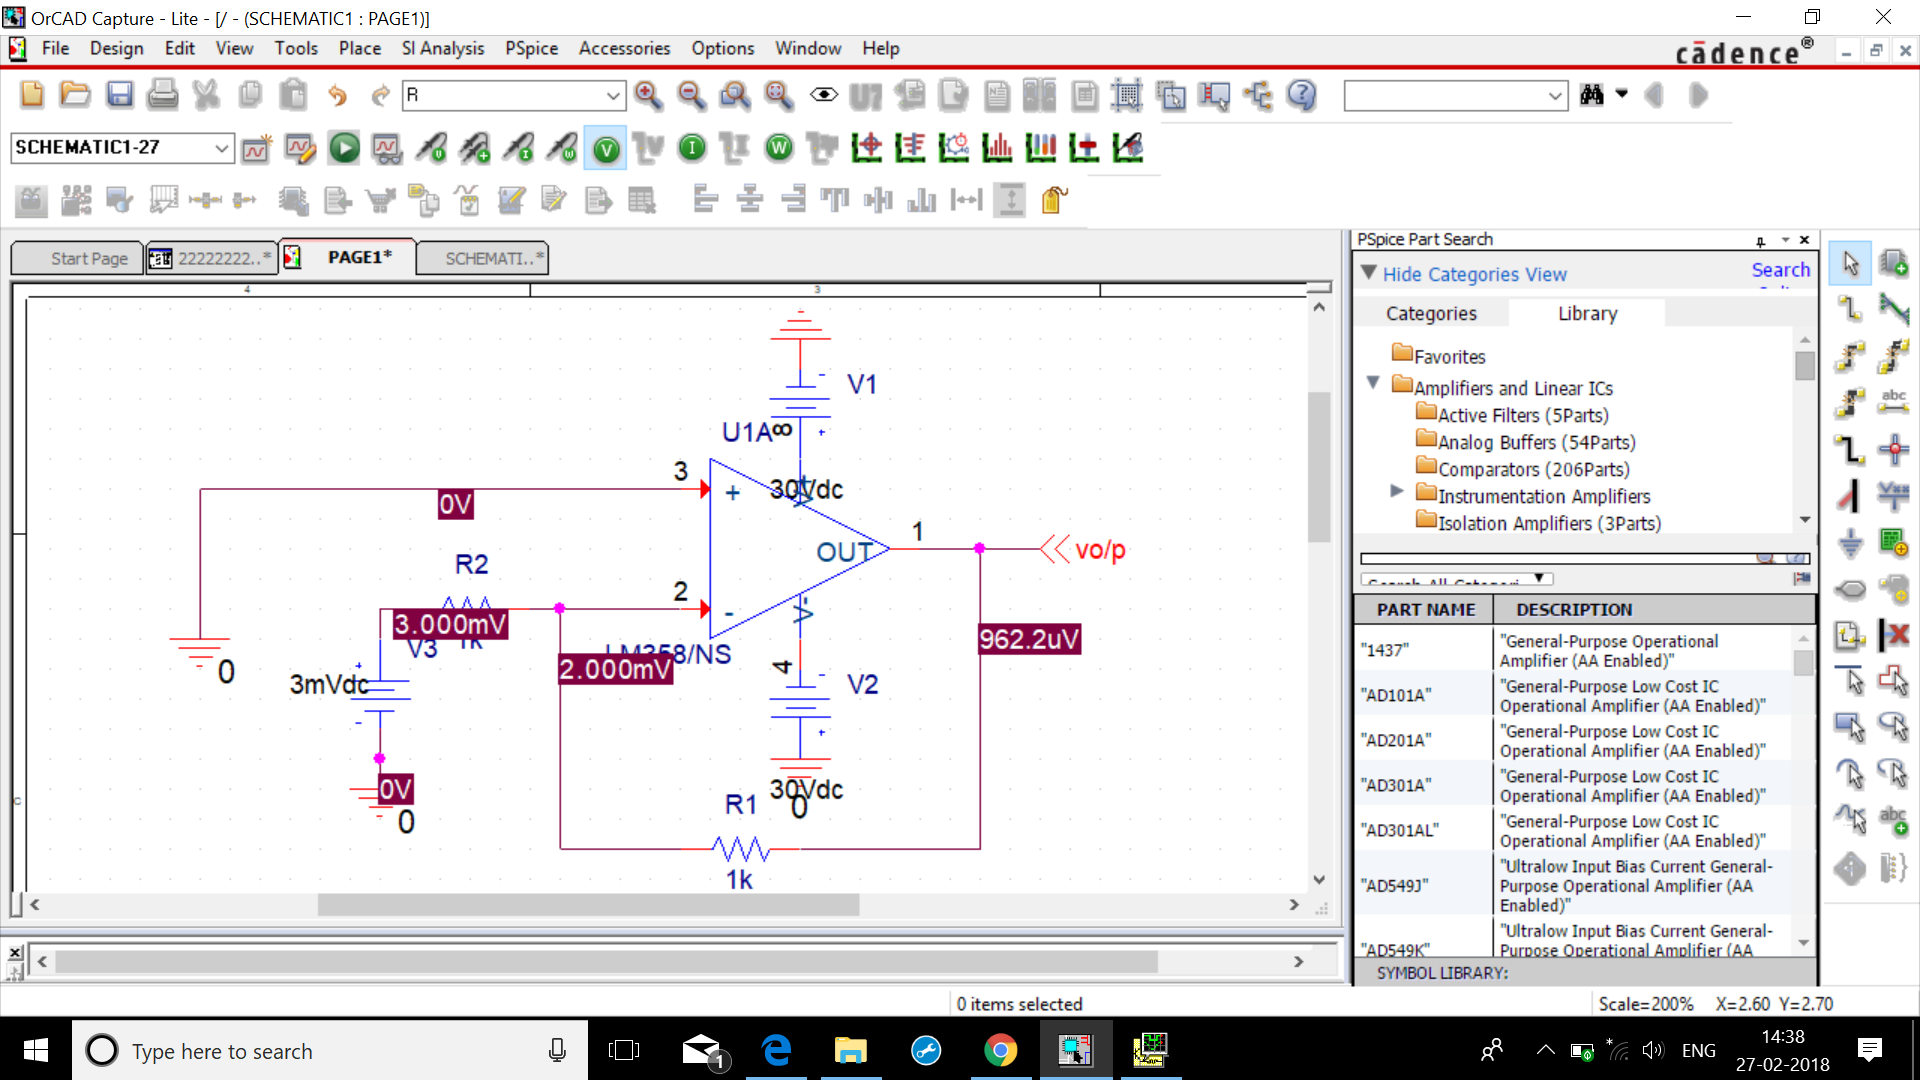
\includegraphics{Q2/offset_volt1}}  
      \centering
      \caption{Circuit Diagram with Voltage Markers }
      \label{fig:offset_volt1}
	\end{figure}
   
\end{homeworkProblem}

\pagebreak

\begin{homeworkProblem}
    
    Design and simulate working of an Instrumentation amplifier for measuring temp change using wheat-stone bridge and instrumentation 	amplifier.
	
    \vspace{5mm}
    \solution \\
    \begin{itemize}
    \item \(R_4\) is the Resistor which is the parameter under consideration. 
    
    
    \item The resistance parameter is varied by graphical conditions.
    The resistor is analogue to the temperature.
    \item Assume, \(R_1,R_2,R_3=100 \Omega\)
    Initially \(R_4=50 \Omega\)
    \\Assume \(Gain(G)=10\)
    \( \therefore R_G=49.4k/(G-1)=5.488k\Omega\)
    \item Due to supply voltage limiting factor the output of instrumentation saturates for \(R_4<72\Omega\)
      
    
    \end{itemize}
    
    \begin{figure}[H] 
      \centering
      \resizebox{12cm}{6cm}{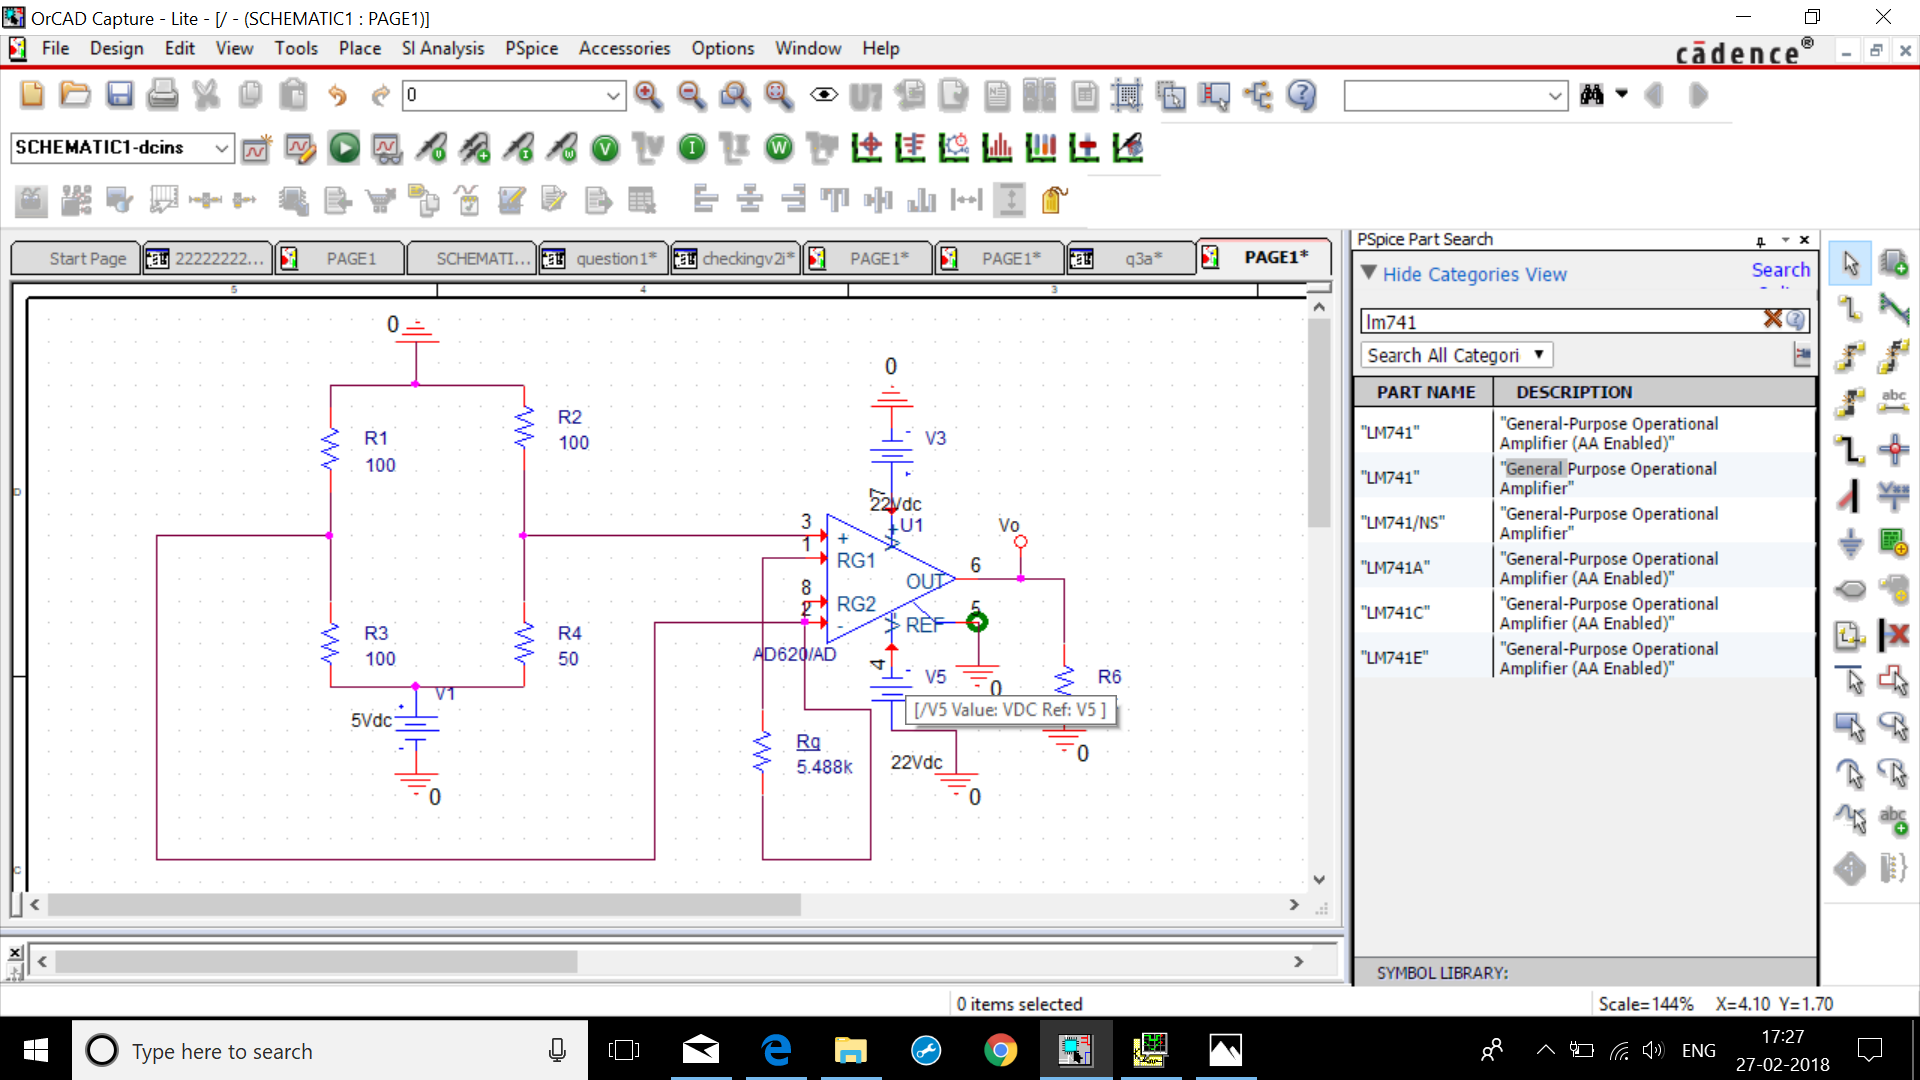
\includegraphics{Q3/circuit}}  
      \centering
      \caption{Circuit Diagram}
      \label{fig:circuit}
	\end{figure}
    
    \begin{figure}[H] 
      \centering
      \resizebox{12cm}{6cm}{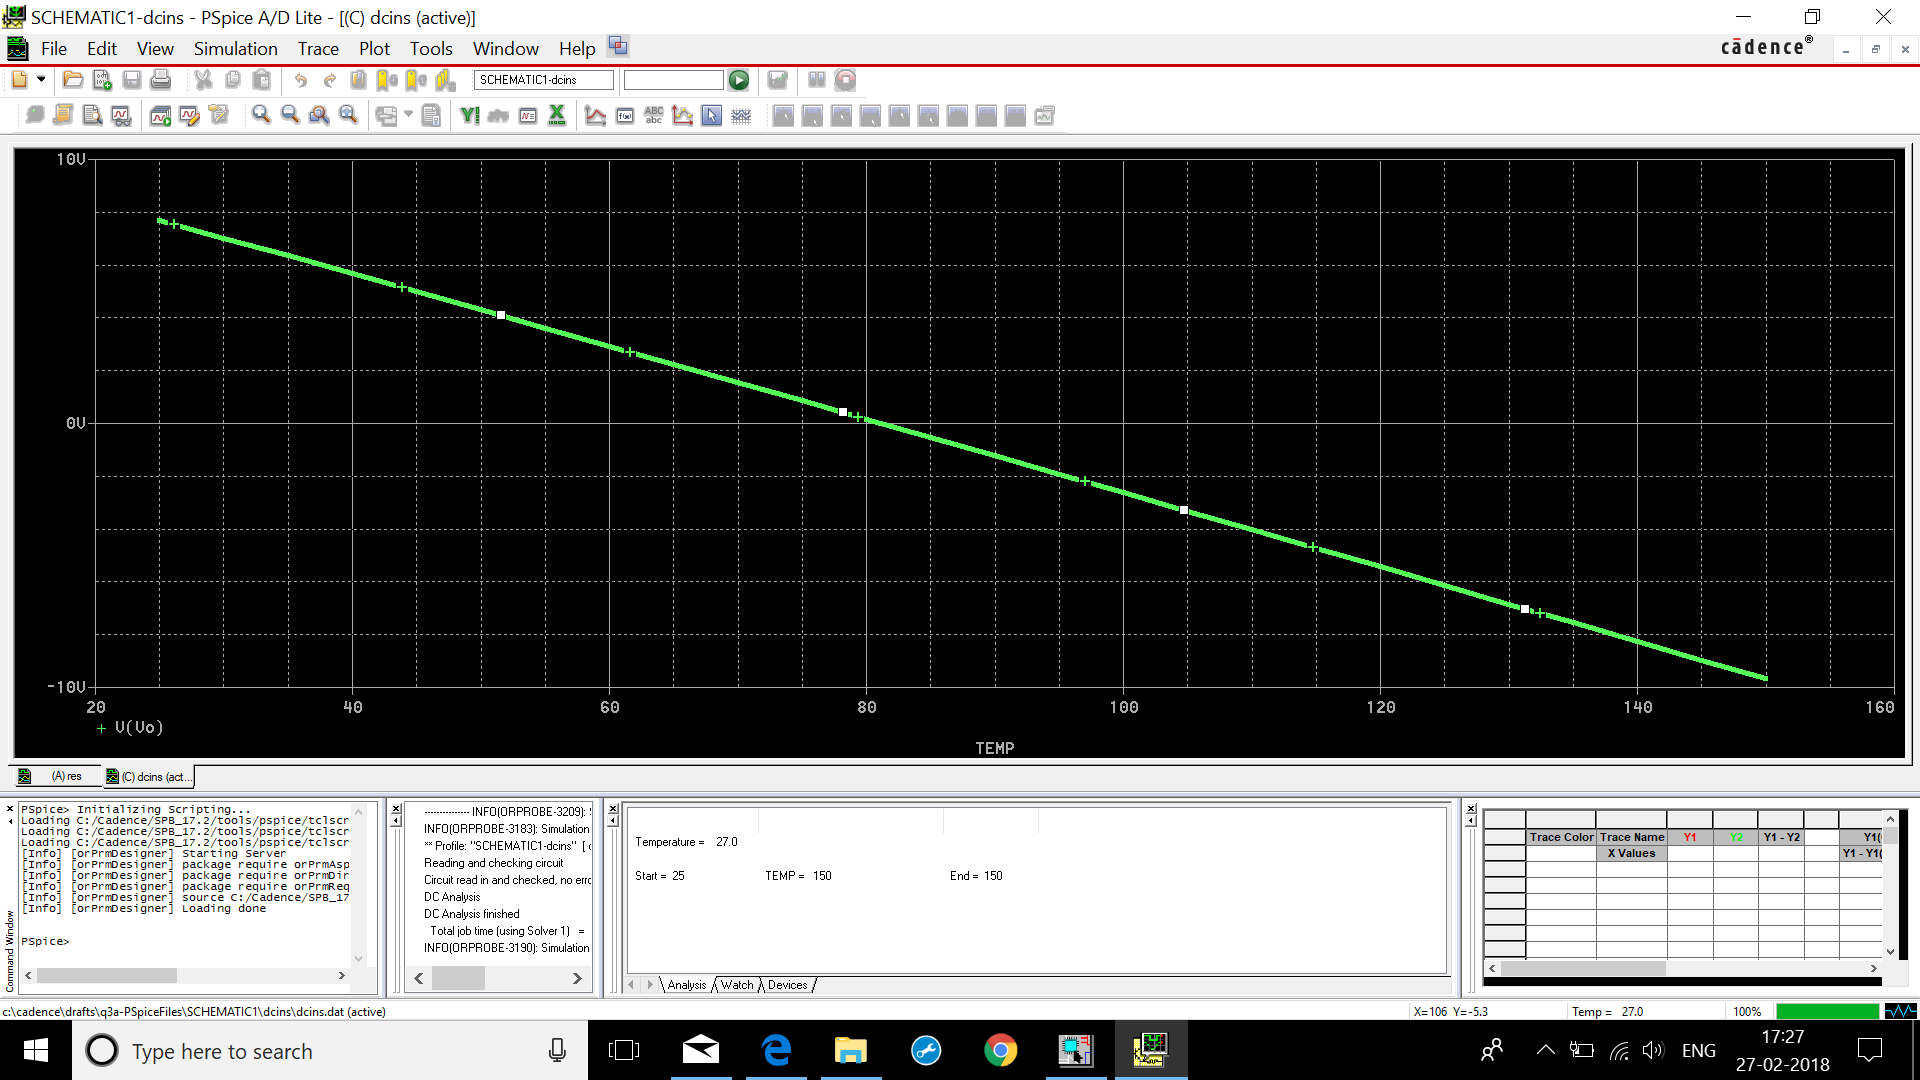
\includegraphics{Q3/graph}}  
      \centering
      \caption{Graph}
      \label{fig:graph}
	\end{figure}
    
\end{homeworkProblem}

\pagebreak

\begin{homeworkProblem}
    
    Design and Simulate a V to I converter with grounded load for an 			application. Measure sensitivity of the circuit.
    
    \vspace{5mm}
    \solution \\
  \begin{itemize}  
    \item The Operational Amplifier used is LM741 and the application specified in this circuit is an LED Tester. 
    \item The LED and the Load Resistance are connected in parallel to each other. 
    \item The Op-Amp is sensing the input voltage thereby producing the output voltage which in turn produces a current flowing through the load.
    \\where, \(I_L=V_i/R_f\)
    \item The LED glows when required amount of current flows through it.The current flowing through the LED is \(0.849\:mA\).
    \end{itemize}
     

	\begin{figure}[H] 
      \centering
      \resizebox{12cm}{6cm}{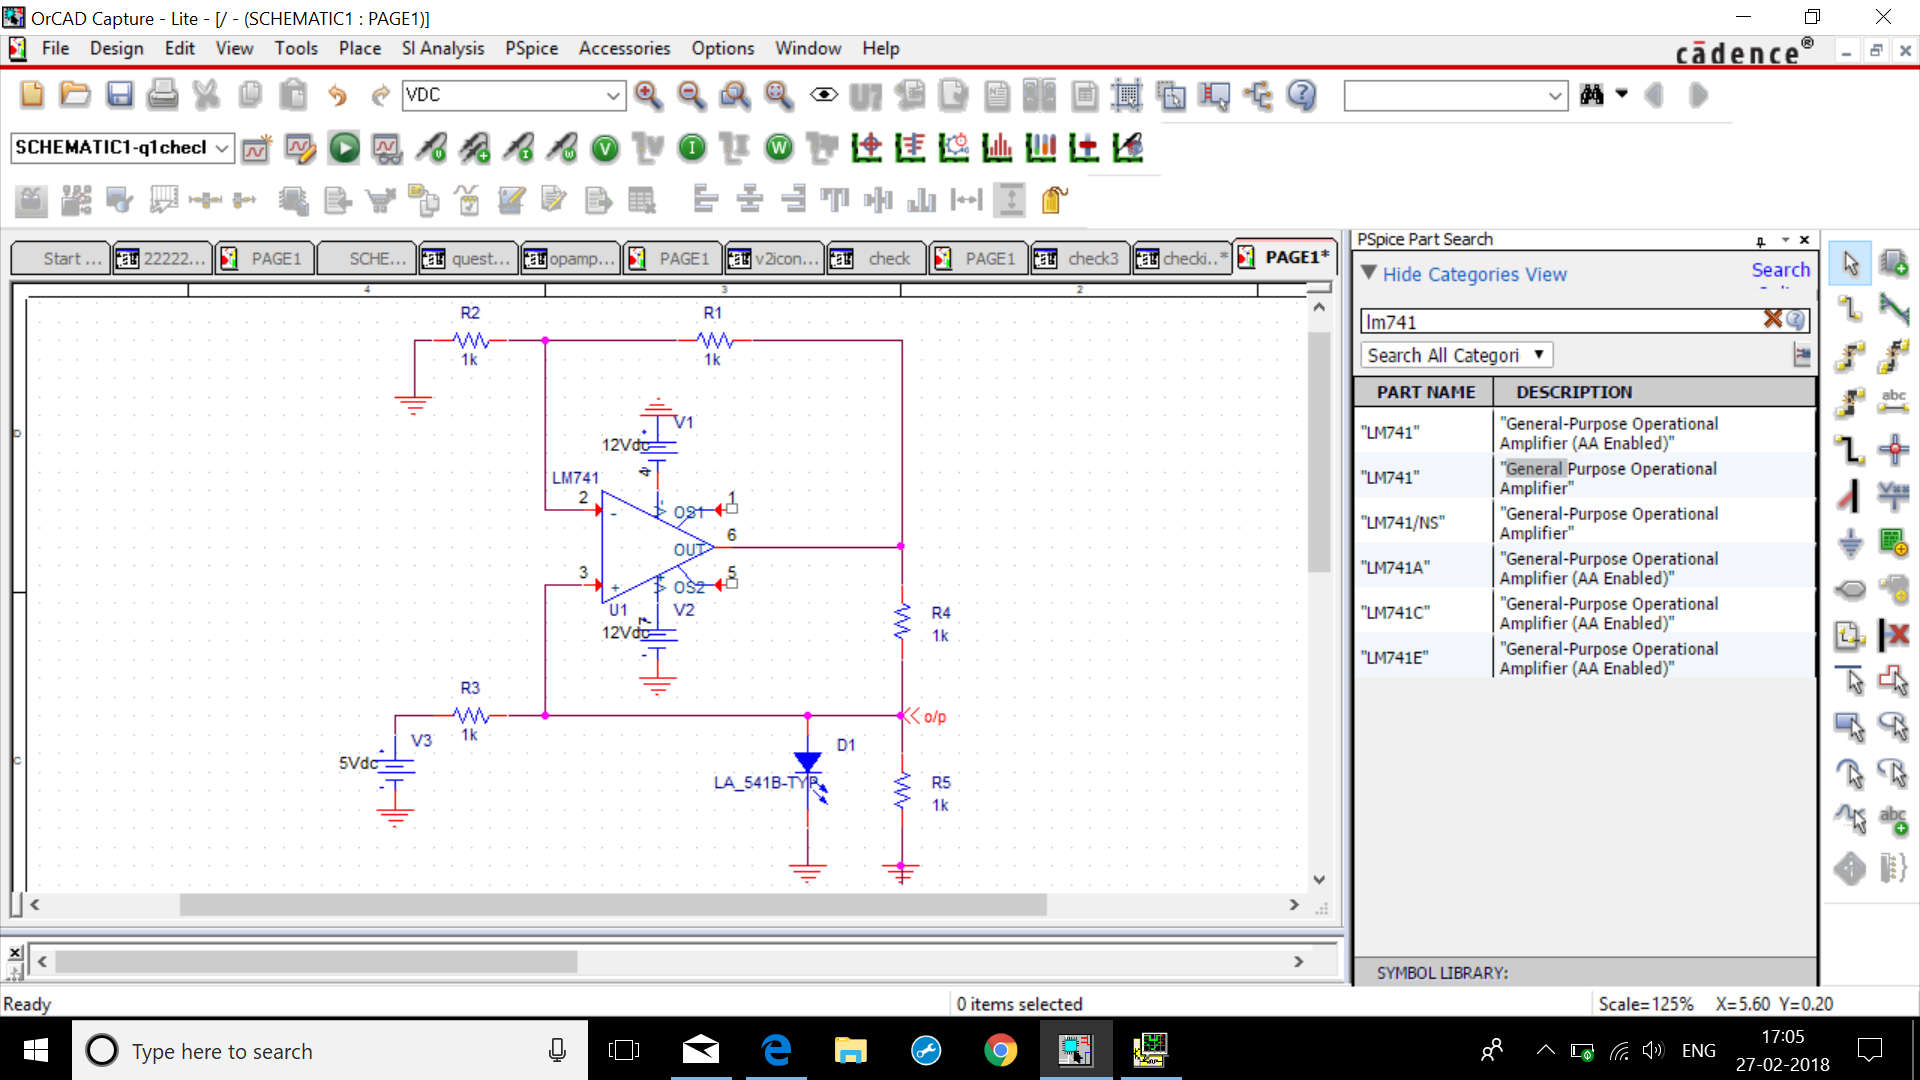
\includegraphics{Q4/circuit}}  
      \centering
      \caption{Circuit Diagram}
      \label{fig:circuit}
	\end{figure}
    
    \begin{figure}[H] 
      \centering
      \resizebox{12cm}{6cm}{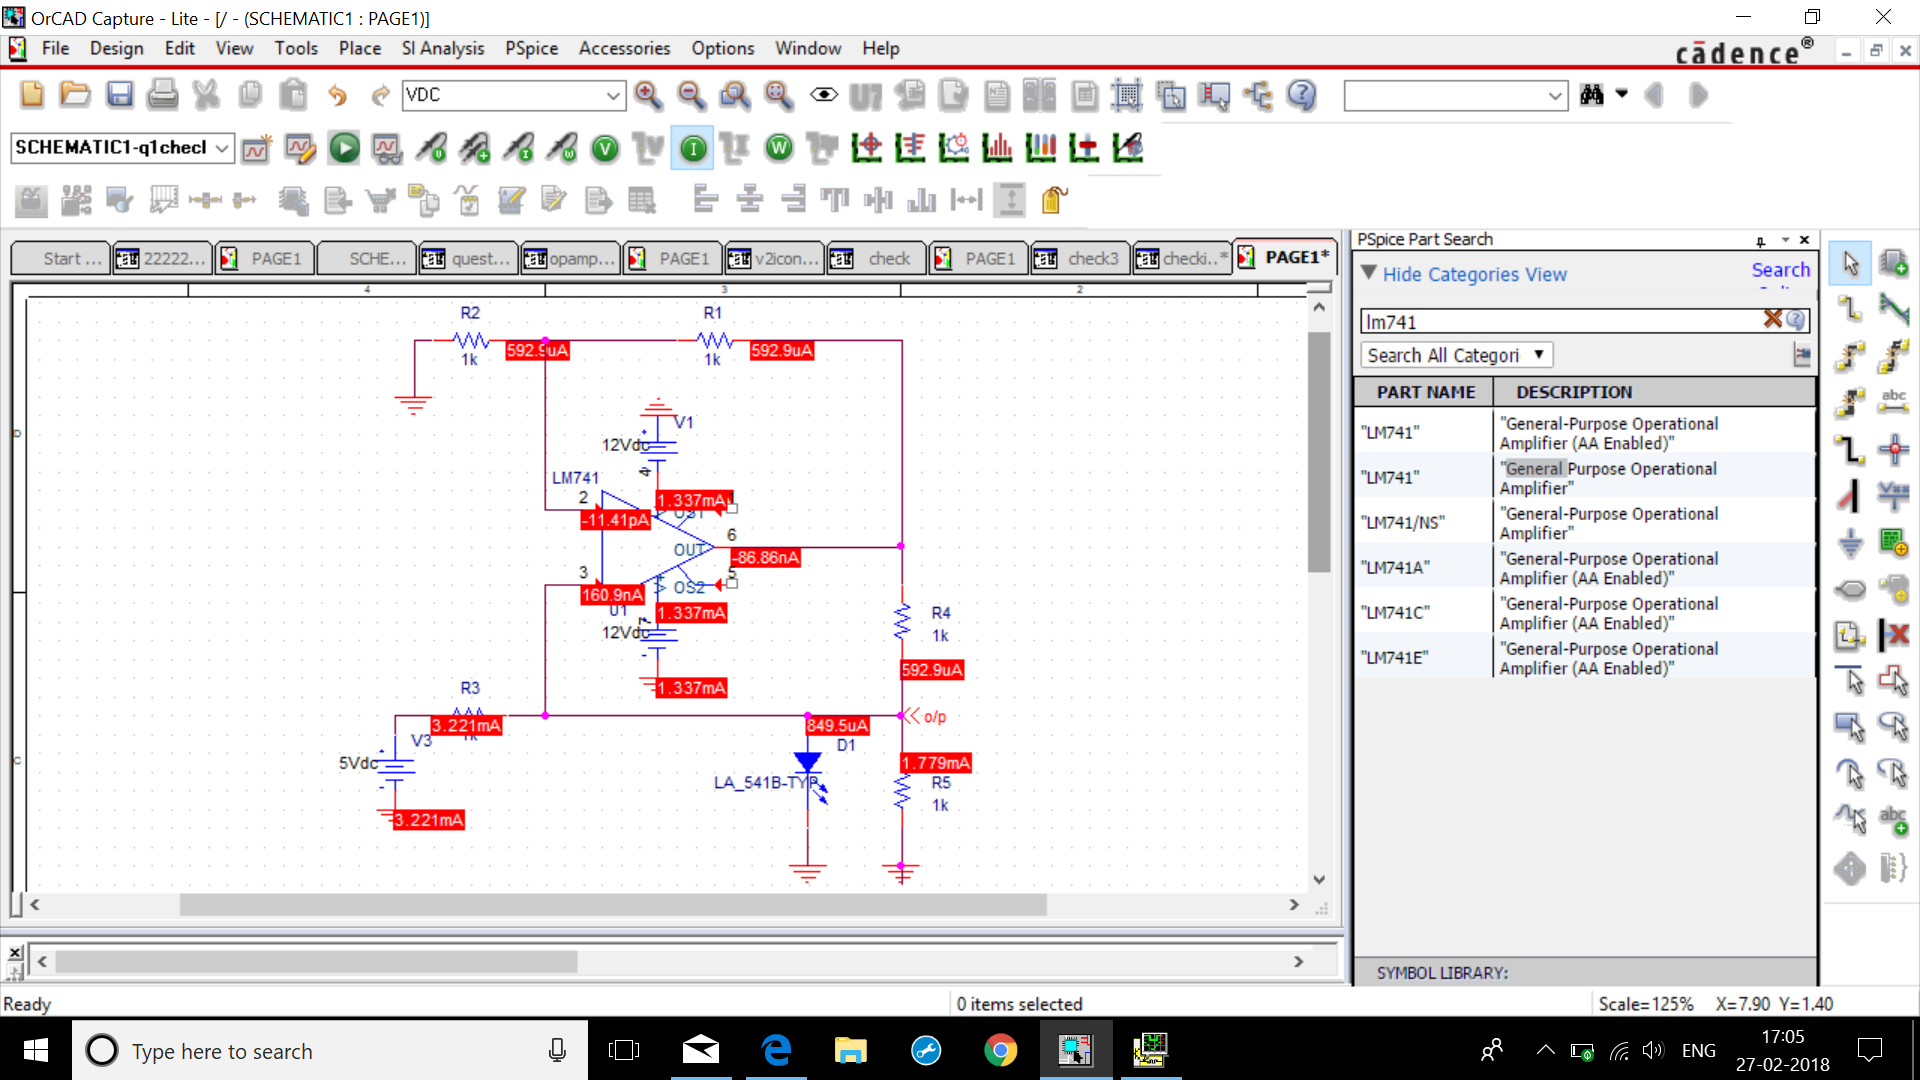
\includegraphics{Q4/circuit_markers}}  
      \centering
      \caption{Circuit Diagram with Current Markers}
      \label{fig:circuit_markers}
	\end{figure}
    
    \begin{figure}[H] 
      \centering
      \resizebox{12cm}{6cm}{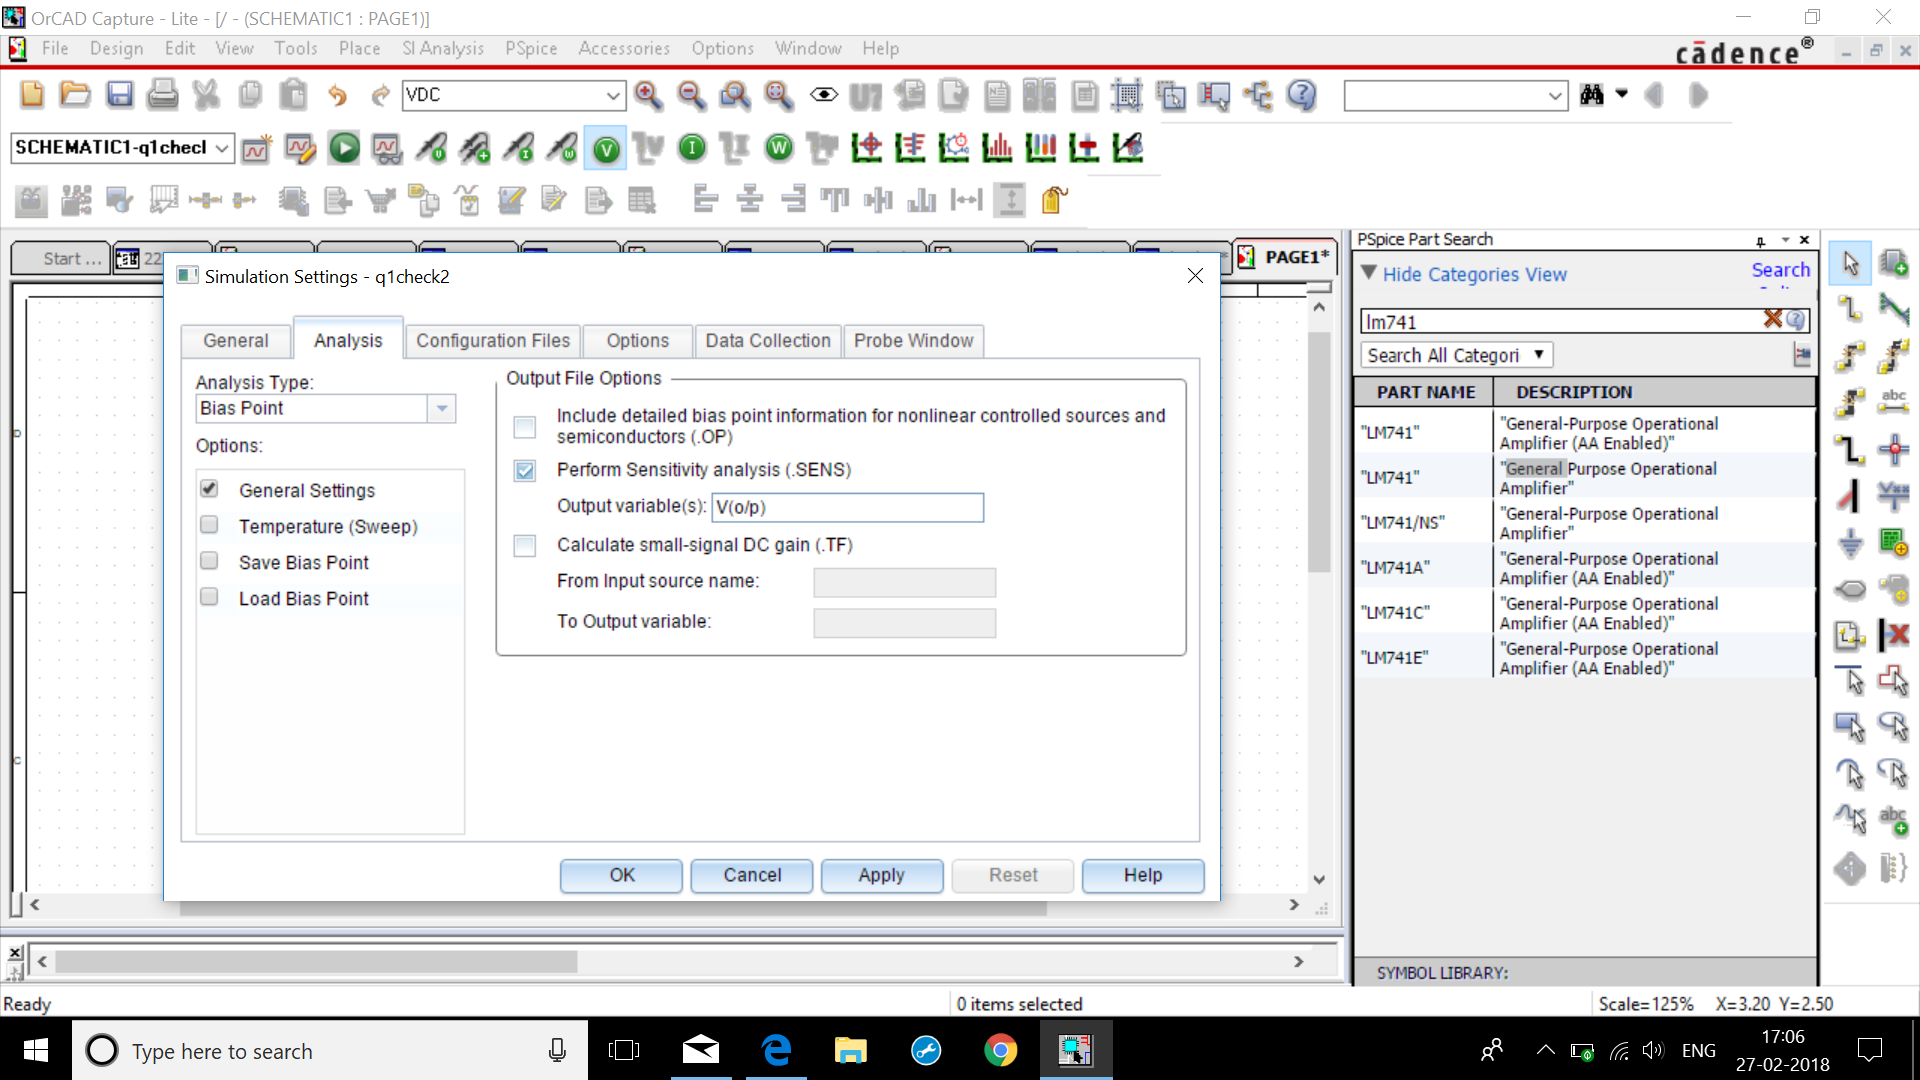
\includegraphics{Q4/sim}}  
      \centering
      \caption{Simulation Settings}
      \label{fig:sim}
	\end{figure}
    
    \begin{figure}[H] 
      \centering
      \resizebox{12cm}{6cm}{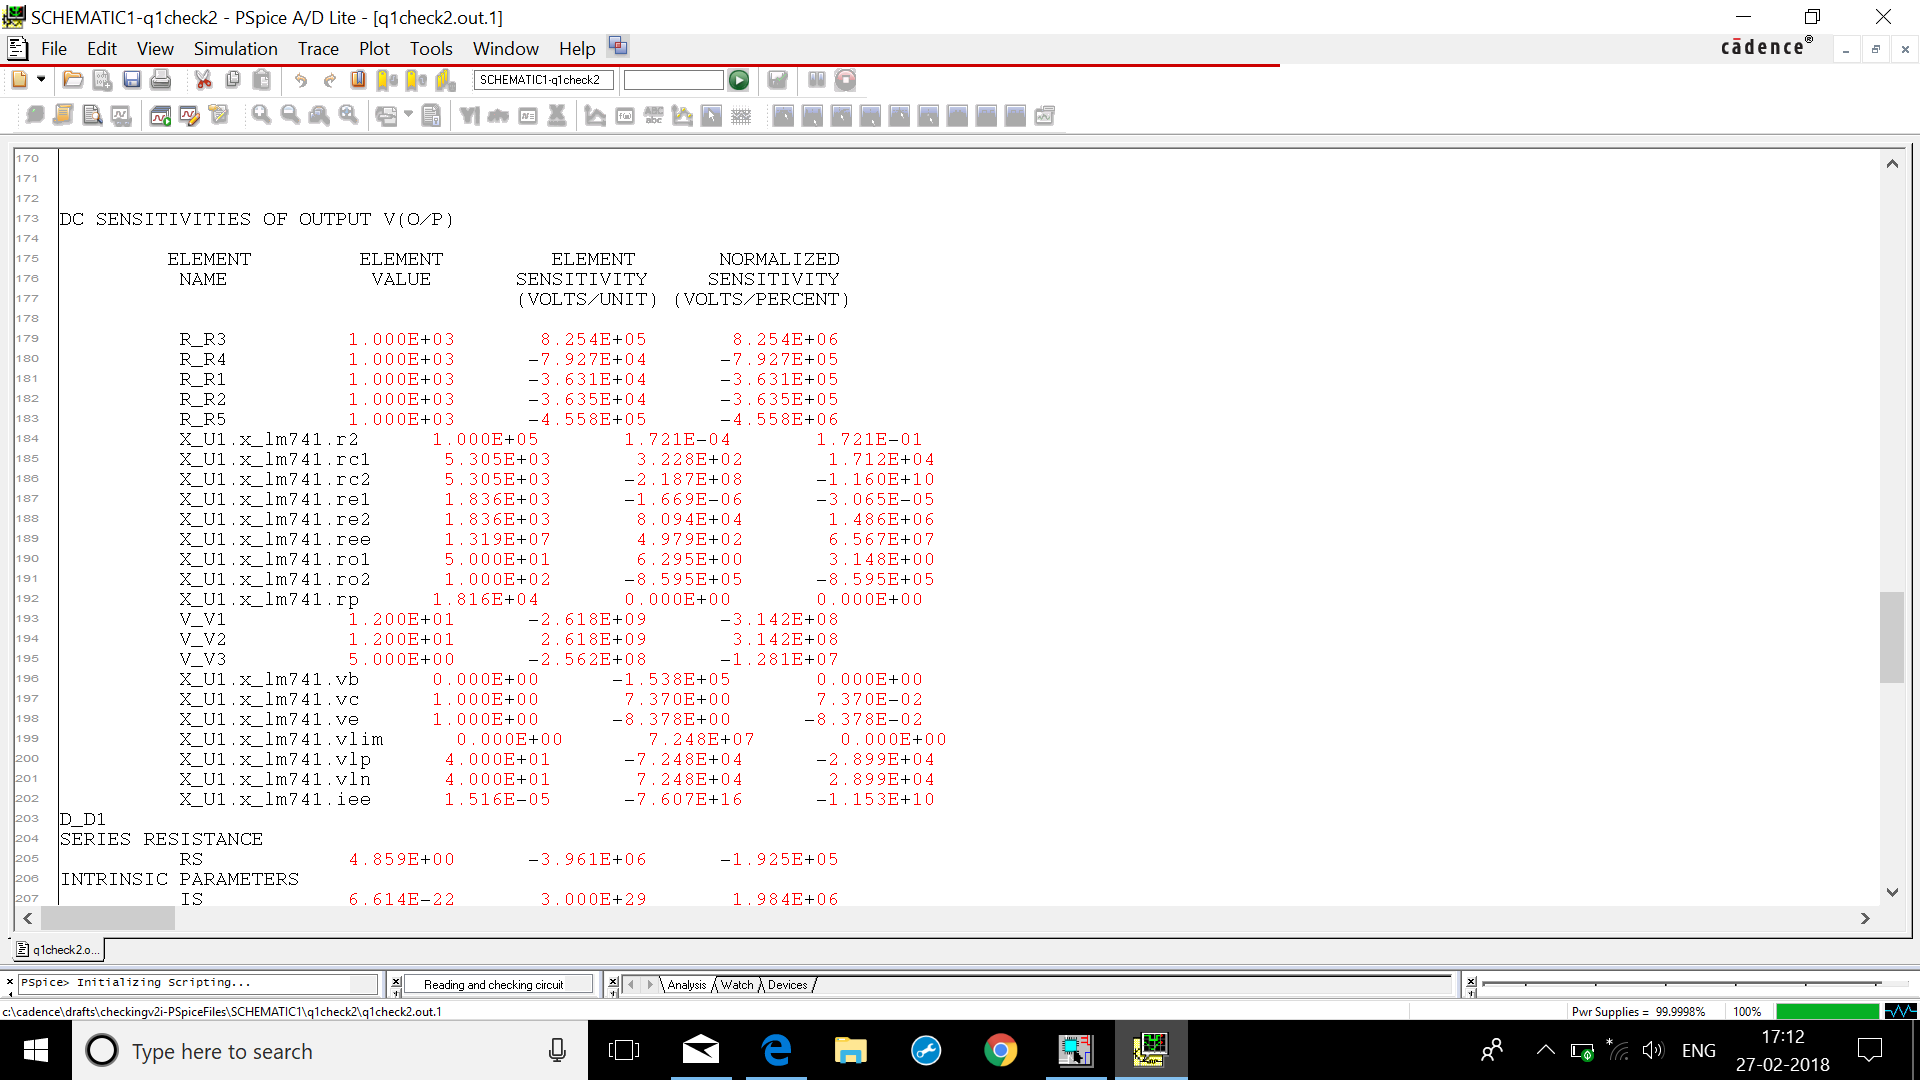
\includegraphics{Q4/output}}  
      \centering
      \caption{Output File}
      \label{fig:output}
	\end{figure}

\end{homeworkProblem}

\pagebreak

\begin{homeworkProblem}
    
    Design and Simulate an experiment to Plot transfer characteristics of 	any practical amp.

	\vspace{5mm}
    \solution
    
    \subsection*{Inverting Open Loop Configuration} 		\label{subsection:origin}

	\begin{itemize}
	\item The practical Operational 		Amplifier LM101A was used for 		this simulation experiment
    \item An input voltage of 0.7 V is provided to the inverting terminal. The non-inverting terminal is grounded.
    \item The circuit was constructed as show in 	Figure \ref{fig:origin}.
	\end{itemize}
	


\begin{figure}[H] 
	\centering
	\resizebox{12cm}{6cm}{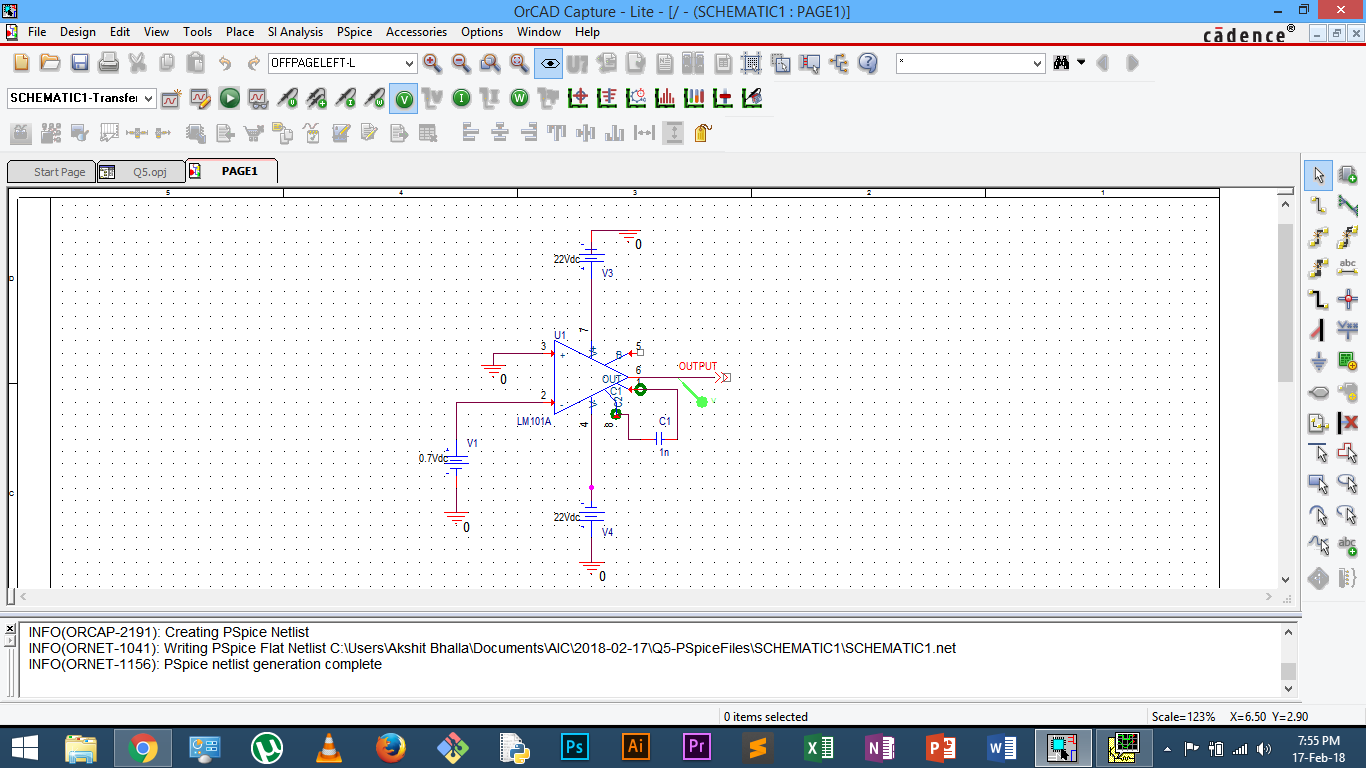
\includegraphics{Q5/origin}}  
	\centering
	\caption{Circuit Diagram}
	\label{fig:origin}
\end{figure}

\begin{figure}[H] 
	\centering
	\resizebox{12cm}{6cm}{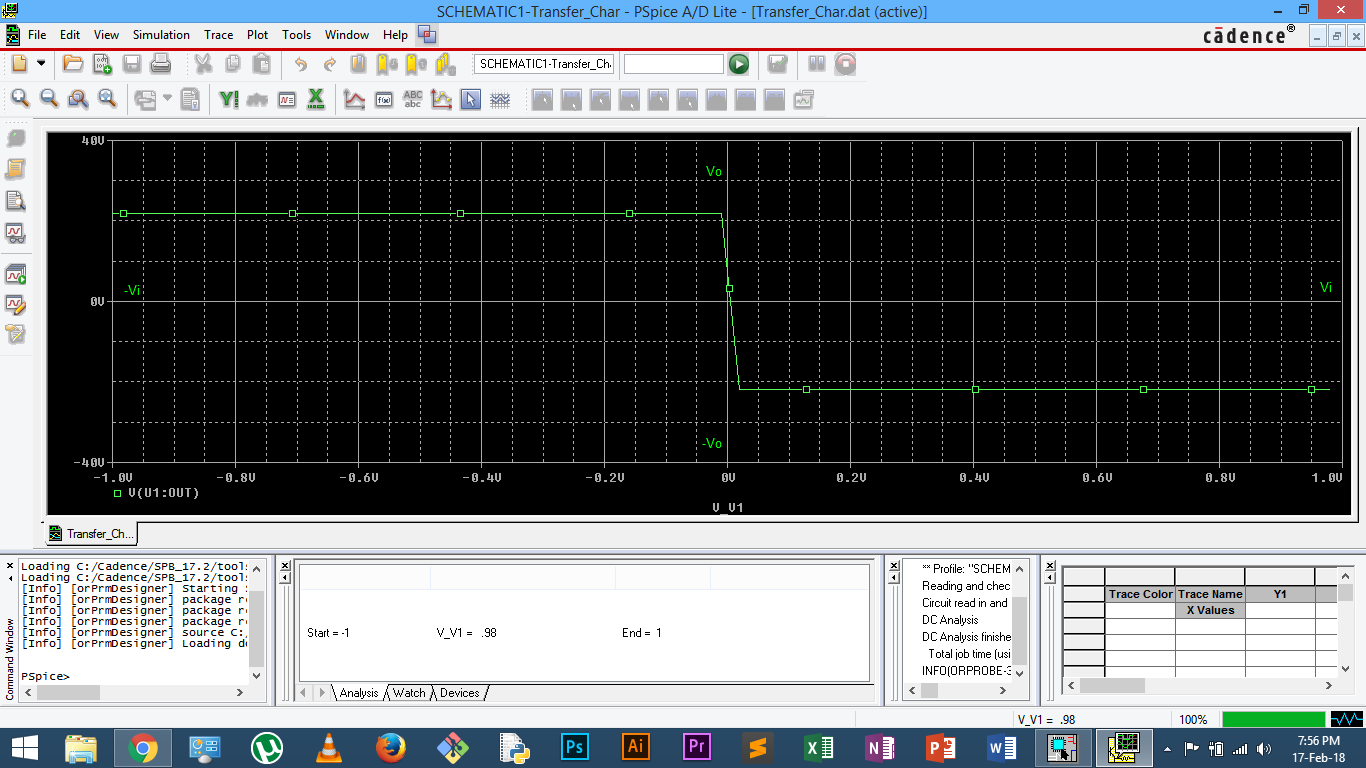
\includegraphics{Q5/origin1}}  
	\centering
	\caption{Transfer Characteristics}
	\label{fig:origin1}
\end{figure}

\pagebreak

\subsection*{Open Loop Configuration with Inverting and Non-Inverting Inputs - 1} \label{subsection:inv}

\begin{itemize}
	\item The practical Operational 		Amplifier LM101A was used for 		this simulation experiment
    \item An input voltage of 0.7 V is provided to the inverting terminal and 0.3 V to the non-inverting terminal. \\ \(V_{inv} > V_{non-inv}\)
    \item The circuit was constructed as show in 	Figure \ref{fig:inv}.
	\end{itemize} 

\begin{figure}[H] 
	\centering
	\resizebox{12cm}{6cm}{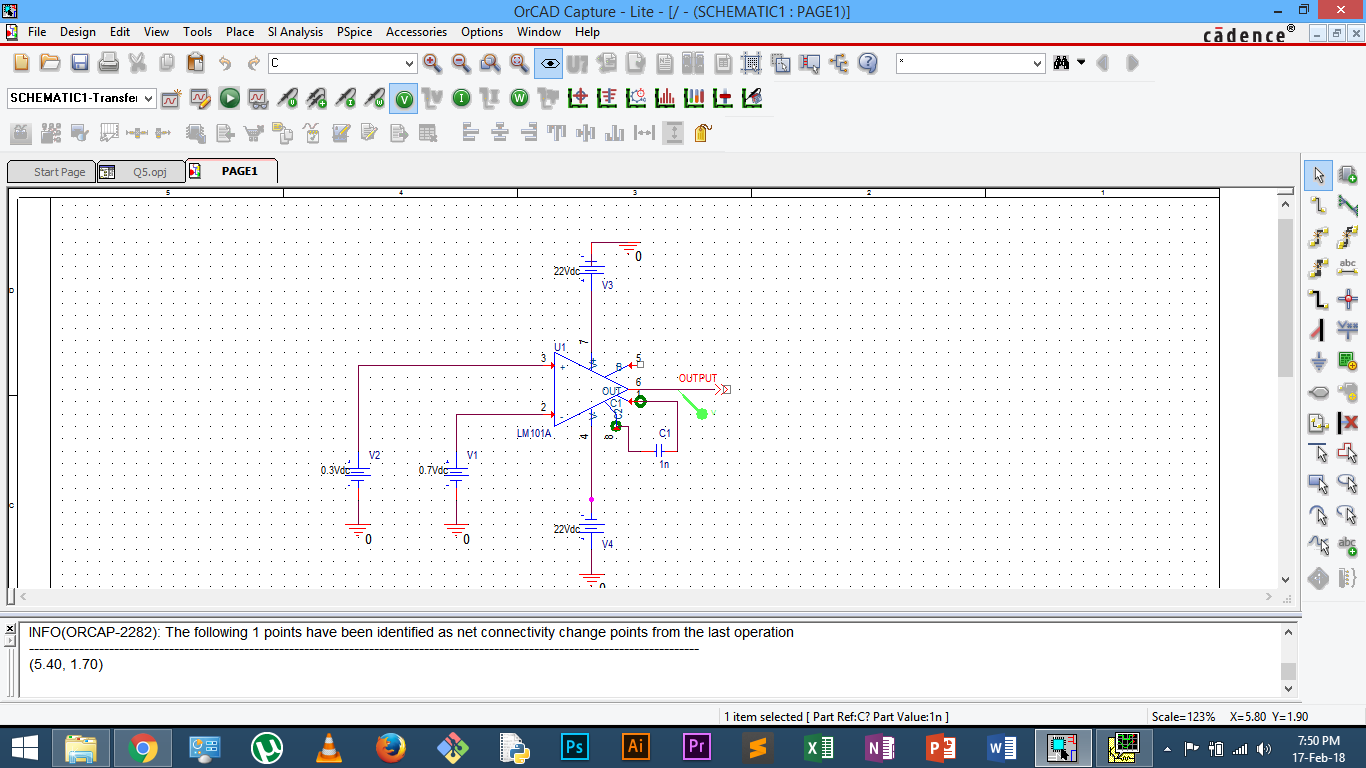
\includegraphics{Q5/inv}}  
	\centering
	\caption{Circuit Diagram}
	\label{fig:inv}
\end{figure}

\begin{figure}[H] 
	\centering
	\resizebox{12cm}{6cm}{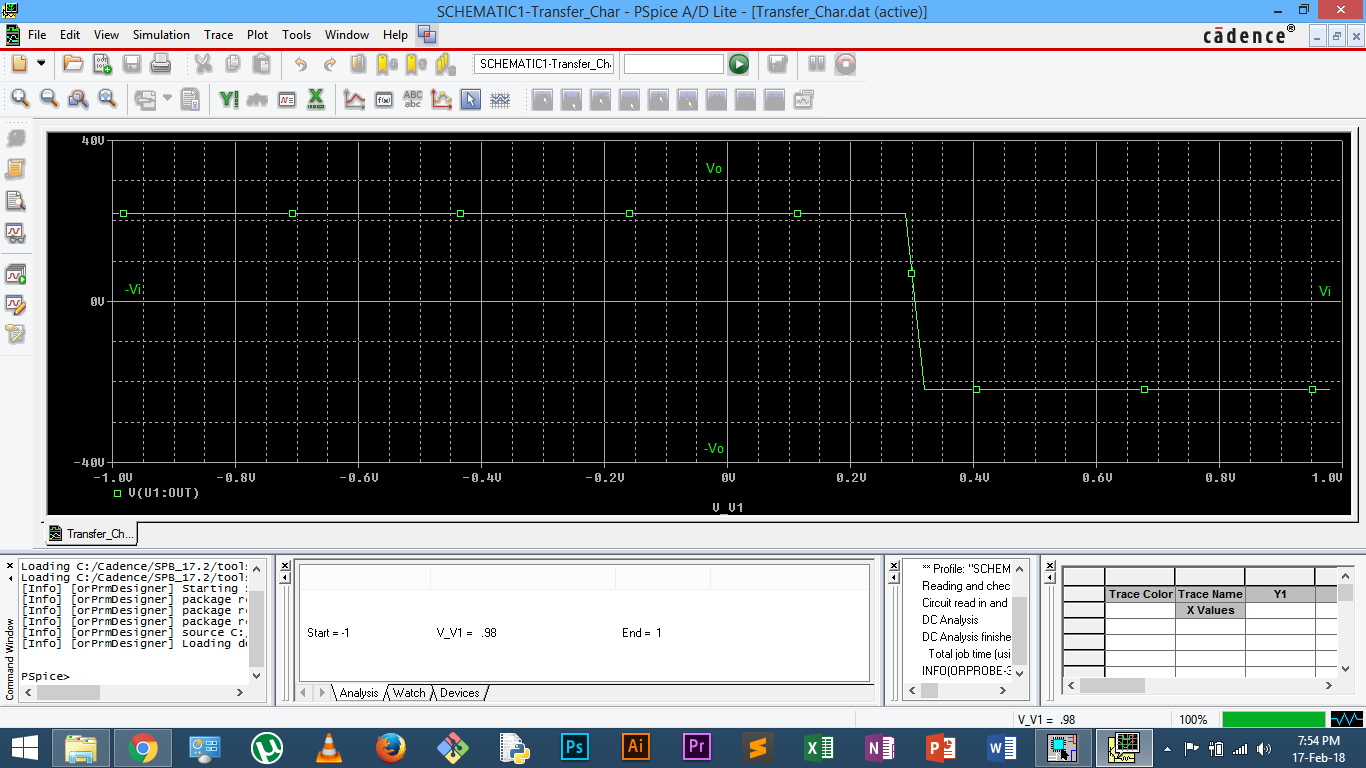
\includegraphics{Q5/inv1}}  
	\centering
	\caption{Transfer Characteristics}
	\label{fig:inv1}
\end{figure}

\pagebreak

\subsection*{Open Loop Configuration with Inverting and Non-Inverting Inputs - 2} \label{subsection:non-inv}

\begin{itemize}
	\item The practical Operational 		Amplifier LM101A was used for 		this simulation experiment
    \item An input voltage of 0.3 V is provided to the inverting terminal and 0.7 V to the non-inverting terminal. \\ \(V_{inv} < V_{non-inv}\)
    \item The circuit was constructed as show in 	Figure \ref{fig:non-inv}.
	\end{itemize} 

\begin{figure}[H] 
	\centering
	\resizebox{12cm}{6cm}{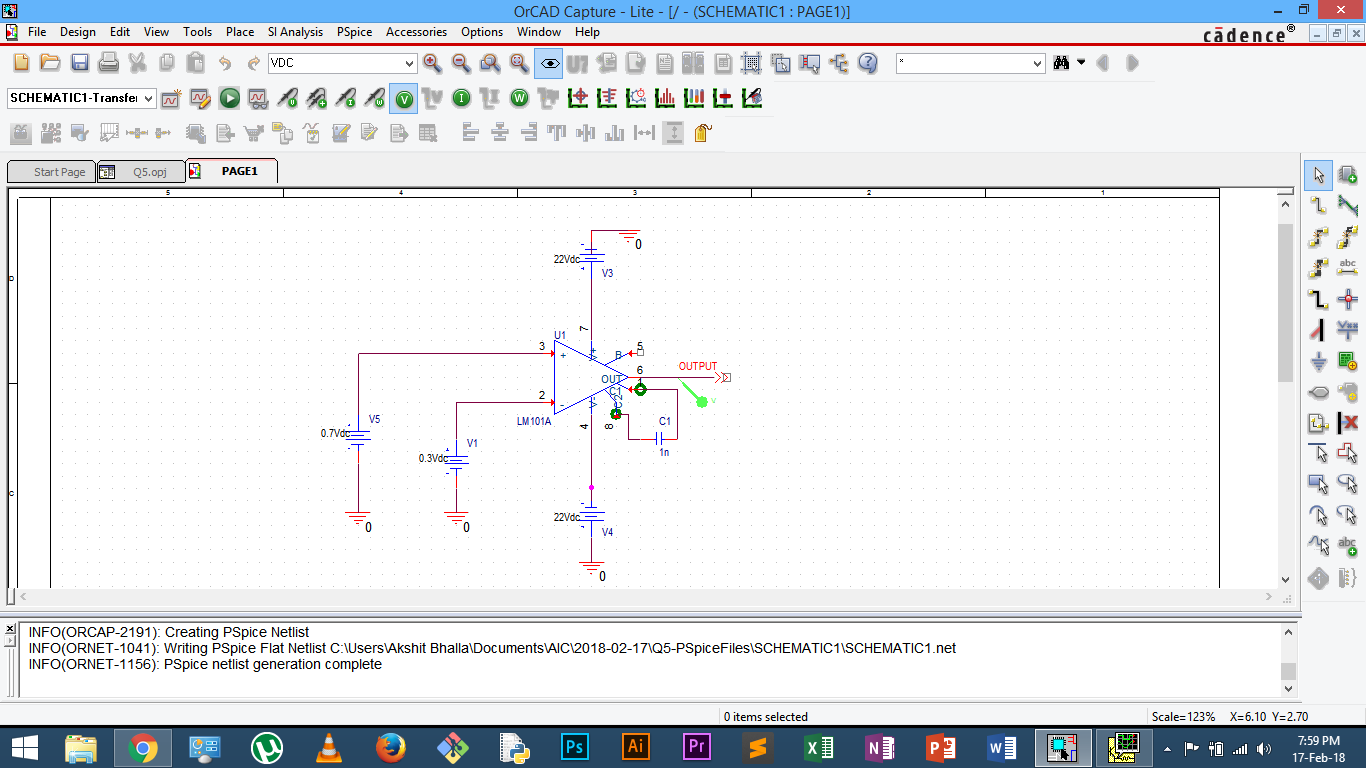
\includegraphics{Q5/non-inv}}  
	\centering
	\caption{Circuit Diagram}
	\label{fig:non-inv}
\end{figure}

\begin{figure}[H] 
	\centering
	\resizebox{12cm}{6cm}{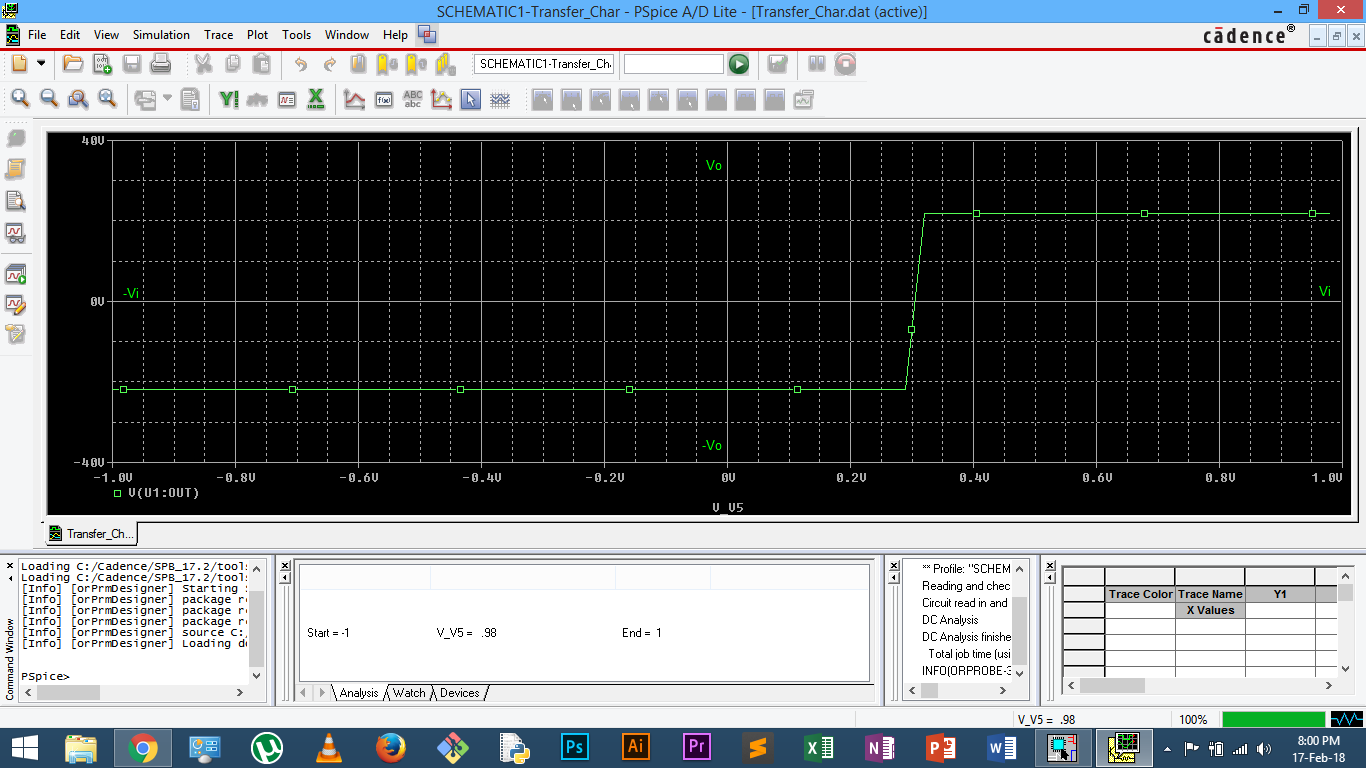
\includegraphics{Q5/non-inv1}}  
	\centering
	\caption{Transfer Characteristics}
	\label{fig:non-inv1}
\end{figure}
    
\end{homeworkProblem}

\pagebreak

{\fontsize{16pt}{16.8pt}\selectfont\textbf{Conclusion}} \\
\begin{itemize}
\item Graphs for open loop gain and closed loop gain could not be merged together on the same graph.
\item The Op-Amp could not be modeled internally to change the pre-defined parameters.

\item The 3 Op-Amp instrumentation amplifier could not be simulated since the maximum number of nodes in the circuit should be \( \approx 75\). Instead a built-in instrumentation amplifier was used.

\end{itemize}


\end{document}
